\chapter{Manual de Usuario\label{extra:manual_de_usuario}}

Este manual pretende ser una guía para la instalación, configuración y uso de la interfaz web para la gestión de sondas de red de altas prestaciones.

\section{Instalación del Servicio Web FPGA\label{extra:manual:instalacionfpga}}

\subsection*{Requisitos}
El servidor que aloje el \gls{servicioweb} \gls{FPGA} debe cumplir los siguientes requisitos:
\begin{itemize}
  \item La \gls{FPGA} para capturar/reproducir tráfico debe estar conectada.
  \item El sistema operativo debe estar basado en una distribución \textit{Debian} \cite{debian} y tener una arquitectura de 64 bits.
  \item La opción por defecto en el gestor de arranque debe ser iniciar con la opción \textit{HugePages} activa.
  \item El usuario \textit{root} debe existir.
\end{itemize}

\subsection*{Instalación}
Para instalar el \gls{servicioweb} \gls{FPGA}, comprobar que se cumplan todos los requisitos y seguir las instrucciones que se describen a continuación:
\begin{enumerate}
  \item Descargar el código fuente del repositorio del proyecto (\href{https://github.com/JSidrach/NetWatcher/archive/master.zip}{\footnotesize{github.com/JSidrach/NetWatcher}}). La instalación se realiza de forma remota, así que no es necesario descargárselo en el propio servidor, aunque sí en un entorno con terminal.
  \item Descomprimir el archivo \textit{.zip}.
  \item Editar el archivo \texttt{./fpga-api/scripts/update\_server.sh}, estableciendo los parámetros \texttt{SERVER\_IP} y \texttt{SERVER\_PATH} como la dirección del servidor remoto que alojará el \gls{servicioweb} \gls{FPGA} y la ruta donde guardar el código, respectivamente.
  \item Situarse en la carpeta \texttt{./fpga-api/}.
  \item Desplegar el servidor ejecutando el siguiente comando:
  
  \texttt{./scripts/update\_server.sh}
  \item Iniciar sesión en el servidor remoto.
  \item Iniciar el \gls{servicioweb} ejecutando el siguiente comando:

  \texttt{sudo service fpga-api start}
  \item Compruebe que el servidor está activo con el siguiente comando:

  \texttt{sudo service fpga-api status}
\end{enumerate}


\section{Configuración del Servicio Web FPGA\label{extra:manual:configfpga}}
Para configurar el \gls{servicioweb} \gls{FPGA}, inicie sesión en el servidor en el que se instaló este servicio. Los distintos parámetros de configuración vienen recogidos en el archivo \texttt{config.js}, dentro de la carpeta raíz del servicio (el contenido de la variable \texttt{SERVER\_PATH}, establecida en la instalación). Edite las distintas variables de este archivo (explicadas en la Tabla \ref{extra:manual:paramsfpga}) para configurar el servicio. No es necesario reiniciar el servicio para que los cambios en el archivo \texttt{config.js} se reflejen en el servidor.

\begin{table}
\centering
\begin{tabular}{|l|l|l|}
\hline
\rowcolor[HTML]{F5F5F5}
\textbf{Variable}   & \textbf{Tipo}    & \textbf{Descripción}                                           \\ \hline
BASE\_PREFIX        & Cadena de texto  & Prefijo base de la \gls{API}                                   \\ \hline
PORT                & Número entero    & Puerto del servicio                                            \\ \hline
MAX\_DELAY          & Número entero    & Retraso máximo entre el \textit{timestamp} de las              \\
                    &                  & peticiones y el \textit{timestamp} del servidor. Si            \\
                    &                  & es menor o igual que 0, no se descartará                       \\ 
                    &                  & ninguna petición basándose en el \textit{timestamp}            \\ \hline
IMPACT\_BIN         & Cadena de texto  & Ruta al ejecutable \texttt{impact} de \textit{Xilinx}          \\ \hline
CAPTURES\_DIR       & Cadena de texto  & Directorio donde se guardarán las \glspl{traza}                \\
                    &                  & (debe acabar en /)                                             \\ \hline
RAID                & Booleano         & Bandera que indica si el \gls{RAID} está activo o              \\
                    &                  & o no. Establezca esta variable como \textit{true}              \\
                    &                  & sólo si \texttt{CAPTURES\_DIR} está sobre un \gls{RAID} y      \\
                    &                  & las variables \texttt{RAID\_DEV} y \texttt{RAID\_DISKS} están  \\
                    &                  & asignadas.                                                     \\ \hline
RAID\_DEV           & Cadena de texto  & Ruta al \gls{RAID}                                             \\ \hline
RAID\_DISKS         & Array de cadenas & Discos físicos del \gls{RAID} (por ejemplo:                    \\
                    &                  & \texttt{/dev/sdc}, \texttt{/dev/sdd}, etc.)                    \\ \hline
\end{tabular}
\caption{Variables de configuración del \gls{servicioweb} \gls{FPGA}}
\label{extra:manual:paramsfpga}
\end{table}


\section{Instalación de la interfaz web\label{extra:manual:instalacionweb}}

\subsection*{Requisitos}
El servidor que aloje la interfaz web debe cumplir los siguientes requisitos:
\begin{itemize}
  \item \textit{Apache httpd} \cite{httpd} debe estar instalado.
  \item La dirección del \gls{servicioweb} \gls{FPGA} debe ser accesible desde este servidor.
\end{itemize}

\subsection*{Instalación}
Para instalar la interfaz web, comprobar que se cumplan todos los requisitos y seguir las instrucciones que se describen a continuación:
\begin{enumerate}
  \item Descargar el código fuente del repositorio del proyecto (\href{https://github.com/JSidrach/NetWatcher/archive/master.zip}{\footnotesize{github.com/JSidrach/NetWatcher}}).
  \item Descomprimir el \textit{.zip} y mueva la carpeta base \textit{NetWatcher} al directorio público de \textit{Apache} (normalmente \texttt{/var/www/html/}).
  \item Situarse en la carpeta base \textit{NetWatcher}.
  \item Instalar los paquetes y librerías necesarios ejecutando el siguiente comando:

  \texttt{sudo ./scripts/build.sh --install}
\end{enumerate}


\section{Configuración de la interfaz web\label{extra:manual:configweb}}

Se puede configurar la interfaz web accediendo en el navegador a la página de configuración, \texttt{IP\_SERVIDOR\_APACHE/NetWatcher/settings}. En esta pantalla (Figura \ref{fig:captura:configuracion}) se puede configurar el idioma, el aspecto visual (tema) y la dirección del \gls{servicioweb} \gls{FPGA}. Para que los cambios se reflejen en la interfaz web es necesario guardarlos. En el resto del manual se presupone que el idioma seleccionado es español.

\begin{figure}[htp!]
  \centering
  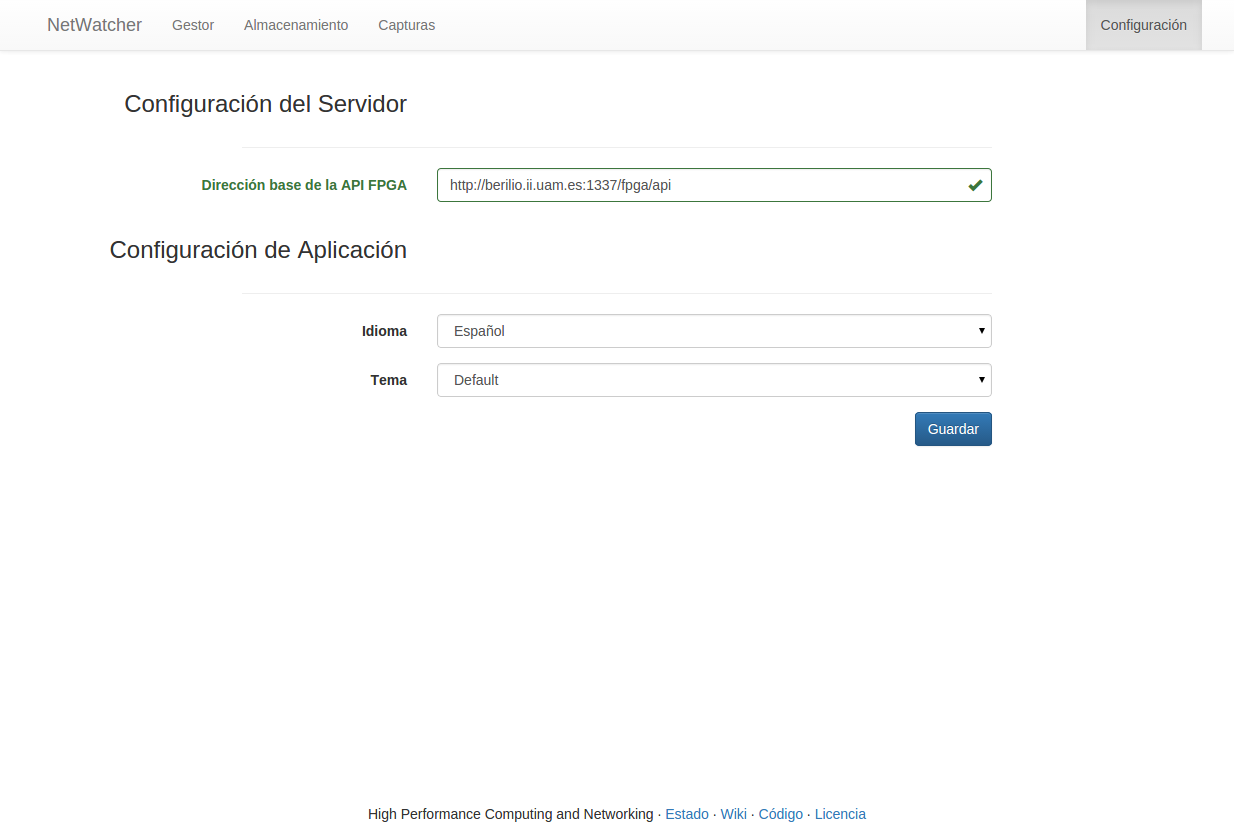
\includegraphics[width=\textwidth,clip=true]{graphics/capturas/configuracion_tema_base}
  \caption{Página de configuración de la interfaz web.}
  \label{fig:captura:configuracion}
\end{figure}


\section{Uso de la aplicación\label{extra:manual:uso}}
Una vez instalados y configurados tanto el \gls{servicioweb} \gls{FPGA} como la interfaz web, ya se puede utilizar la interfaz. Esta interfaz se puede usar desde cualquier navegador, y tanto en ordenador como en móvil. Todas las pantallas tienen las mismas barras de navegación.

Desde la barra de navegación superior se puede acceder a las siguientes pantallas:
\begin{itemize}
  \item \textbf{Gestor}: administración de la \gls{FPGA}.
  \item \textbf{Almacenamiento}: estadísticas de almacenamiento y del \gls{RAID}, si está activo.
  \item \textbf{Capturas}: gestión de las \glspl{traza} almacenadas.
  \item \textbf{Configuración}: explicada en la sección \ref{extra:manual:configweb}.
\end{itemize}

La barra de navegación inferior contiene los siguientes elementos:
\begin{itemize}
  \item \textbf{Estado}: enlace a la pantalla con estado actual del sistema.
  \item \textbf{Wiki}: enlace a la documentación del proyecto.
  \item \textbf{Código}: enlace al repositorio de código del proyecto.
  \item \textbf{Licencia}: despliega la licencia del proyecto.
\end{itemize}

Adicionalmente, se puede acceder a la documentación interna autogenerada del proyecto (en inglés) mediante las siguientes rutas relativas a la dirección base de la interfaz web:
\begin{itemize}
  \item \textbf{Documentación del \gls{servicioweb} \gls{FPGA}}: \texttt{/docs-back-end/}.
  \item \textbf{Documentación de la interfaz web}: \texttt{/docs-front-end/}.
\end{itemize}

En las siguientes subsecciones se explica cómo utilizar las principales pantallas interactivas de la interfaz web.


\subsection{Gestor\label{extra:manual:gestor}}

En esta pantalla se controla el estado de la \gls{FPGA}. El contenido de esta pantalla, y por tanto las acciones disponibles, cambian según el estado actual de la \gls{FPGA}.

Si la \gls{FPGA} no ha sido inicializada, la pantalla de gestión permitirá seleccionar un modo en el que inicializarla:
\begin{itemize}
  \item \textbf{Reproductor}: permite reproducir \glspl{traza} en formato \gls{simple}.
  \item \textbf{Capturador}: permite capturar tráfico web, almacenándolo en una \gls{traza} en formato \gls{simple}.
\end{itemize}

Para elegir un modo basta con pulsar uno de los dos botones de la interfaz (ver Figura \ref{fig:captura:gestionseleccion}). Esta elección de modo no es definitiva, ya que se puede cambiar de modo en cualquier momento siempre que la \gls{FPGA} no esté capturando o reproduciendo tráfico.

\begin{figure}[!htp]
  \centering
  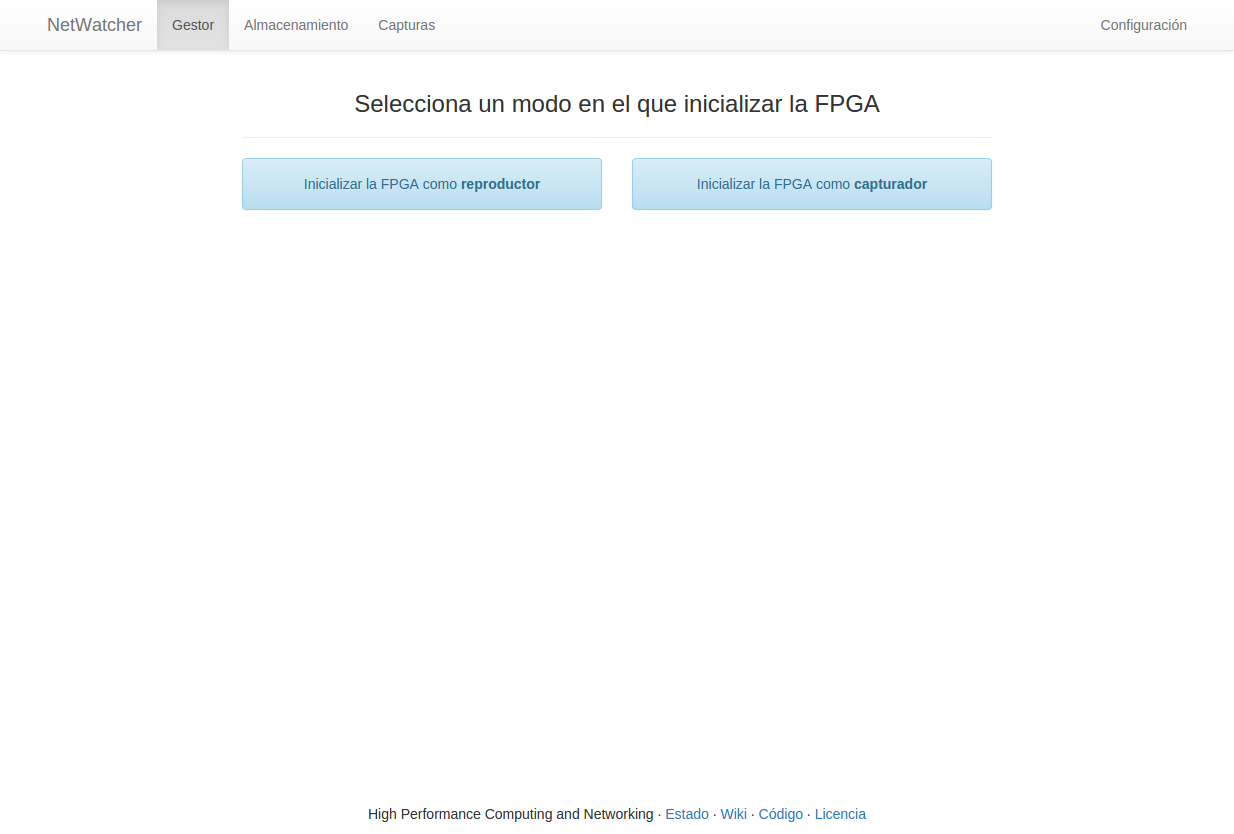
\includegraphics[width=\textwidth,clip=true]{graphics/capturas/gestor_seleccion}
  \caption{Página de gestión - selección de modo.}
  \label{fig:captura:gestionseleccion}
\end{figure}

Una vez seleccionado un modo, un cuadro de diálogo muestra el progreso de la inicialización: programando la \gls{FPGA}, reiniciando el servidor y montando la \gls{FPGA} (ver Figura \ref{fig:captura:gestionprogreso}).

\begin{figure}[!htp]
  \centering
  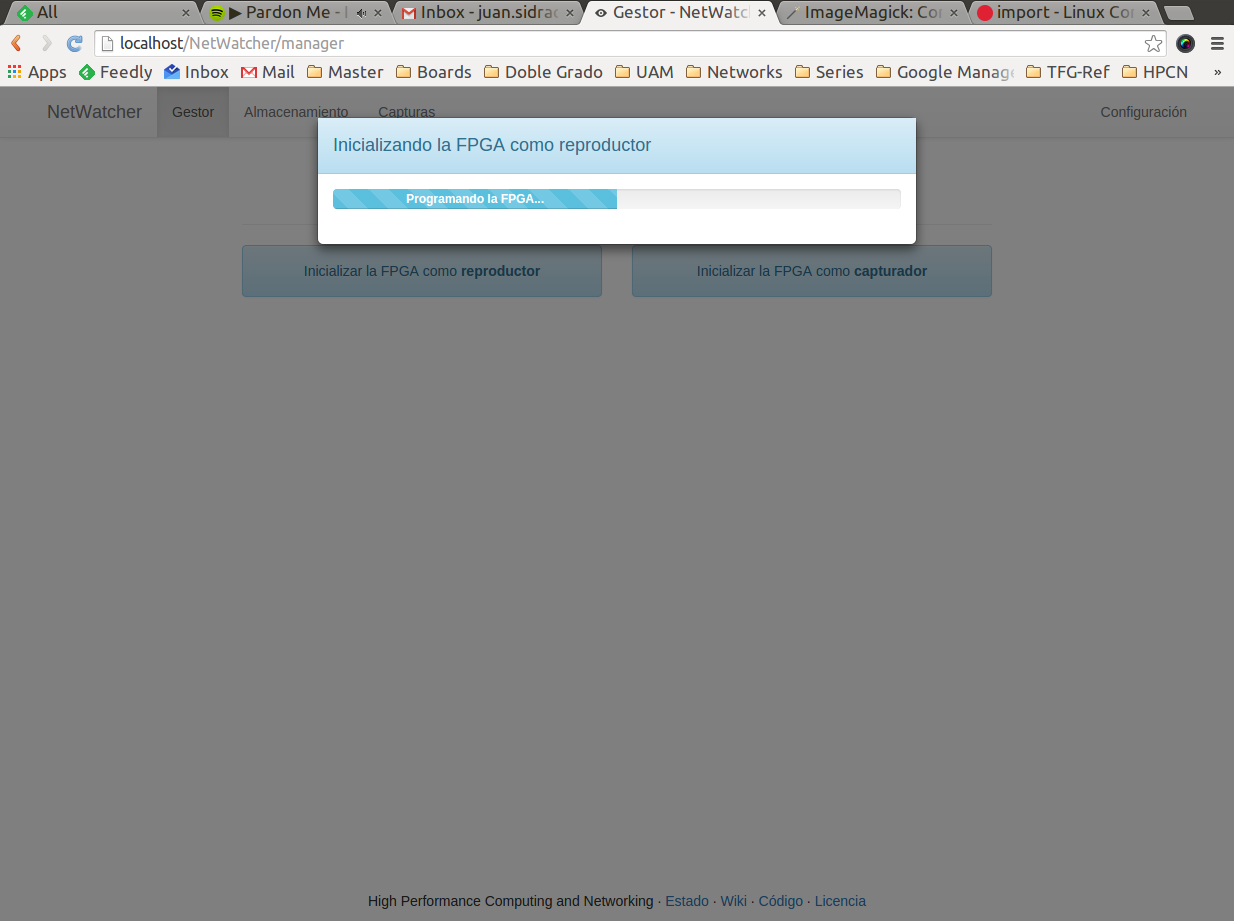
\includegraphics[width=\textwidth,clip=true]{graphics/capturas/gestor_seleccion_progreso}
  \caption{Página de gestión - selección de modo en progreso.}
  \label{fig:captura:gestionprogreso}
\end{figure}

Si la \gls{FPGA} ha sido inicializada en modo capturador, la pantalla de gestión mostrará un formulario en el que se configurarán los parámetros de una captura (ver Figura \ref{fig:captura:gestioncapturar}). Este formulario contiene los siguientes campos, todos ellos obligatorios:
\begin{itemize}
  \item \textbf{Nombre de la nueva \gls{traza}}: nombre que tendrá la \gls{traza} en la que se almacenará el tráfico capturado, en formato \gls{simple}.
  \item \textbf{Bytes a capturar}: número total de bytes que se capturarán, y su unidad (Bytes, KB, MB, GB).
  \item \textbf{Puerto a capturar}: puerto del que se capturará el tráfico entrante (0, 1, 2, 3).
\end{itemize}

Los dos primeros campos se iluminarán en verde cuando sean introducidos correctamente y en rojo cuando sean incorrectos. Cuando todos los campos sean válidos se activará el botón de \textit{Empezar}, y si se pulsa la \gls{FPGA} comenzará a capturar tráfico con los parámetros indicados.

También es posible, en vez de capturar tráfico, volver a seleccionar modo pulsando el correspondiente enlace debajo del formulario.

\begin{figure}[!htp]
  \centering
  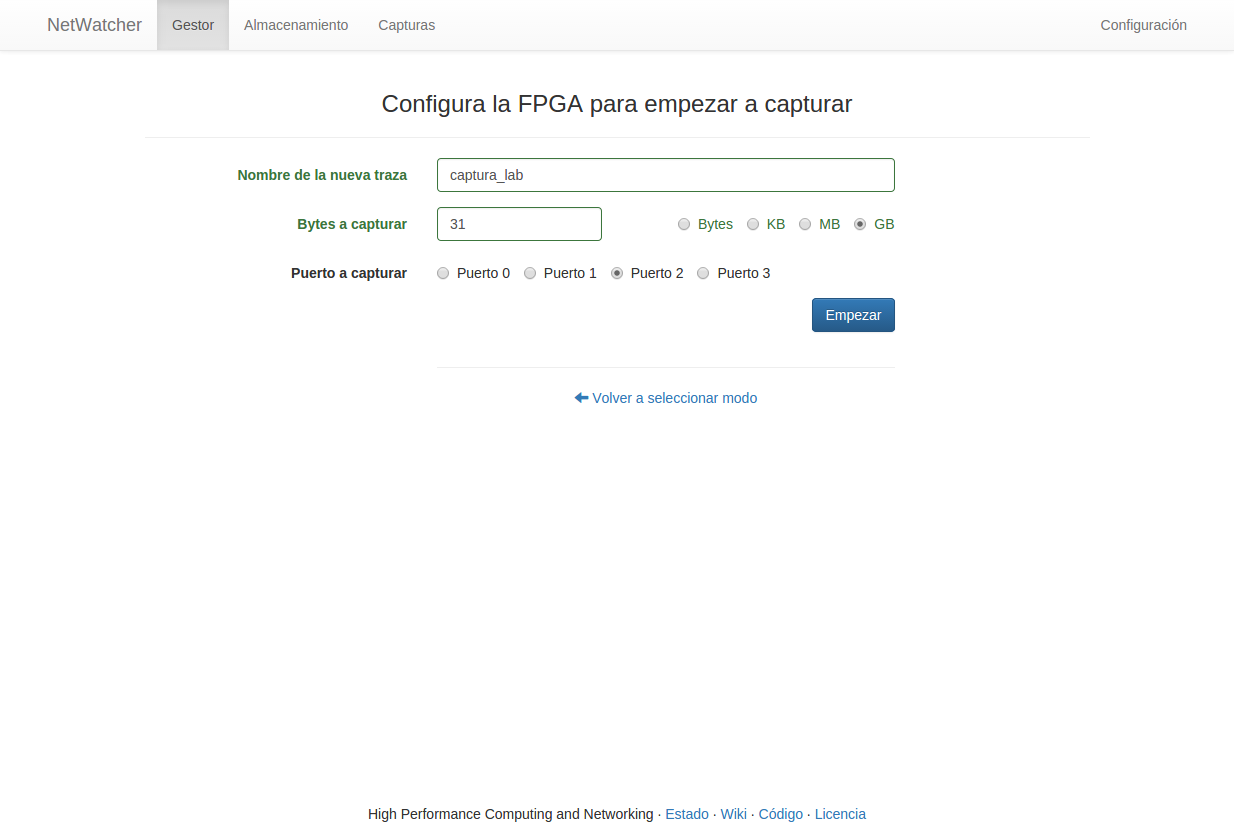
\includegraphics[width=\textwidth,clip=true]{graphics/capturas/gestor_capturar}
  \caption{Página de gestión - capturar tráfico.}
  \label{fig:captura:gestioncapturar}
\end{figure}

Si la \gls{FPGA} está capturando tráfico, la pantalla de gestión mostrará el progreso de la captura en curso (ver Figura \ref{fig:captura:gestioncapturando}). Se podrán visualizar las siguientes estadísticas de la captura en curso:
\begin{itemize}
  \item \textbf{Nombre de la traza}: nombre de la \gls{traza} en la que se está almacenando el tráfico capturado, en formato \gls{simple}.
  \item \textbf{Puerto}: puerto del que se está capturando el tráfico entrante.
  \item \textbf{Tiempo transcurrido}: contador del tiempo que ha transcurrido desde que se inició la captura.
  \item \textbf{Bytes Capturados}: número de bytes que se han capturado ya.
  \item \textbf{Bytes Totales}: número total de bytes a capturar.
  \item \textbf{Ratio Medio}: velocidad media a la que se está capturando (estimación a partir de los bytes capturados y el tiempo transcurrido).
  \item \textbf{Ratio Actual}: velocidad a la que se ha capturado el tráfico desde la última actualización.
\end{itemize}

Se puede detener la captura en curso pulsando el botón de \textit{Parar la captura}, y se borrará lo almacenado hasta el momento en la \gls{traza}.

\begin{figure}[!htp]
  \centering
  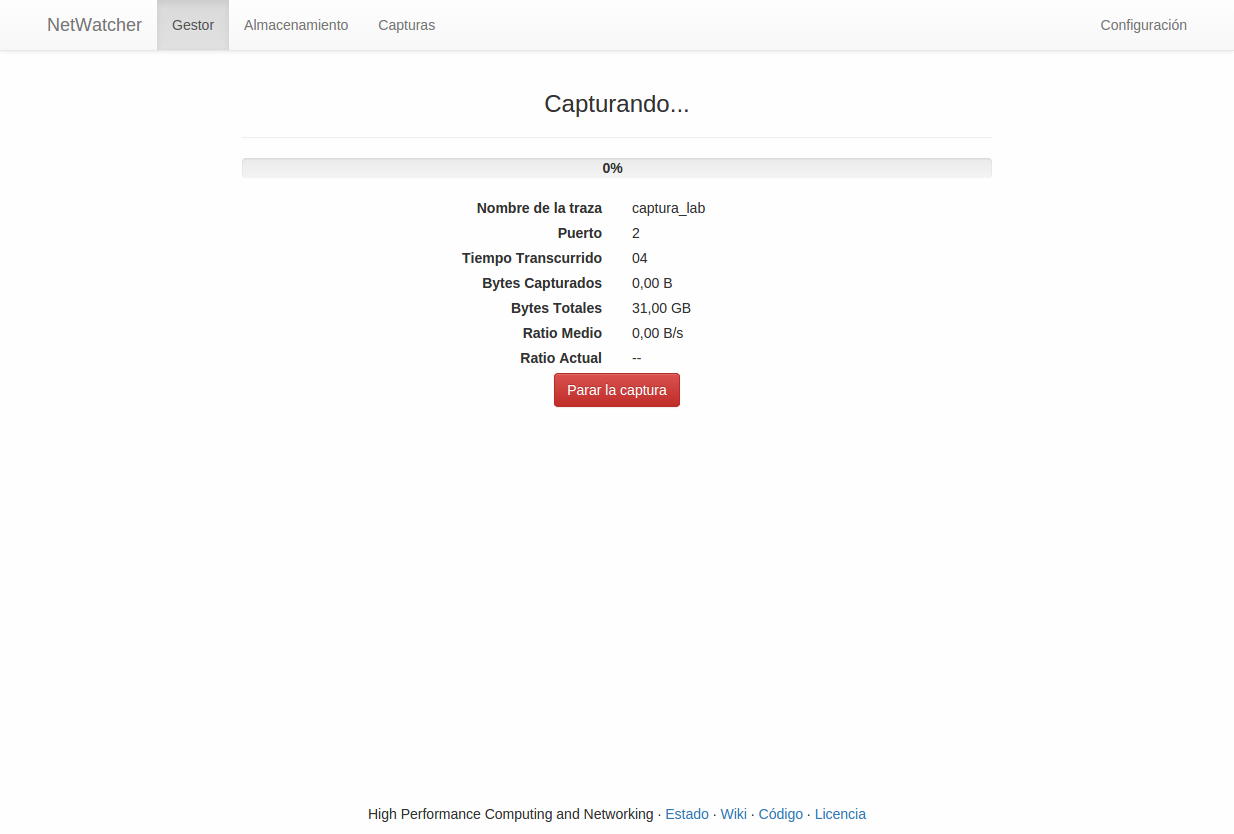
\includegraphics[width=\textwidth,clip=true]{graphics/capturas/gestor_capturando}
  \caption{Página de gestión - capturando tráfico.}
  \label{fig:captura:gestioncapturando}
\end{figure}

Si la \gls{FPGA} ha sido inicializada en modo reproductor, la pantalla de gestión mostrará una tabla y un formulario (ver Figura \ref{fig:captura:gestionreproducir}). La tabla contiene una fila por cada \gls{traza} disponible, con su nombre, tipo (\gls{simple}), tamaño y fecha. Además, una barra superior asociada a esta tabla permite controlar el contenido de la misma mediante las siguientes acciones (de izquierda a derecha): activar la actualización automática de las \glspl{traza} disponibles, buscar una \gls{traza} por su nombre y actualizar manualmente las \glspl{traza} disponibles. Pulsando sobre una fila de la tabla se seleccionará la \gls{traza} correspondiente para su reproducción. Por otra parte, el formulario contiene los siguientes campos:
\begin{itemize}
  \item \textbf{Reproducir la \gls{traza} en bucle}: si se habilita, la \gls{traza} se reproducirá en un bucle infinito.
  \item \textbf{Máscara de salida}: conjunto de puertos a los que se reproducirá la \gls{traza} (0, 0-1, 0-1-2, 0-1-2-3).
  \item \textbf{Interframe Gap}: pausa temporal entre paquetes (si se deshabilita, tasa original con la que se capturó la \gls{traza}).
\end{itemize}

Cuando se haya seleccionado una traza de la tabla y todos los campos del formulario sean válidos se activará el botón de \textit{Empezar}, y si se pulsa la \gls{FPGA} comenzará a reproducir la \gls{traza} seleccionada con los parámetros indicados.

También es posible, en vez de reproducir tráfico, volver a seleccionar modo pulsando el correspondiente enlace debajo del formulario.

\begin{figure}[!htp]
  \centering
  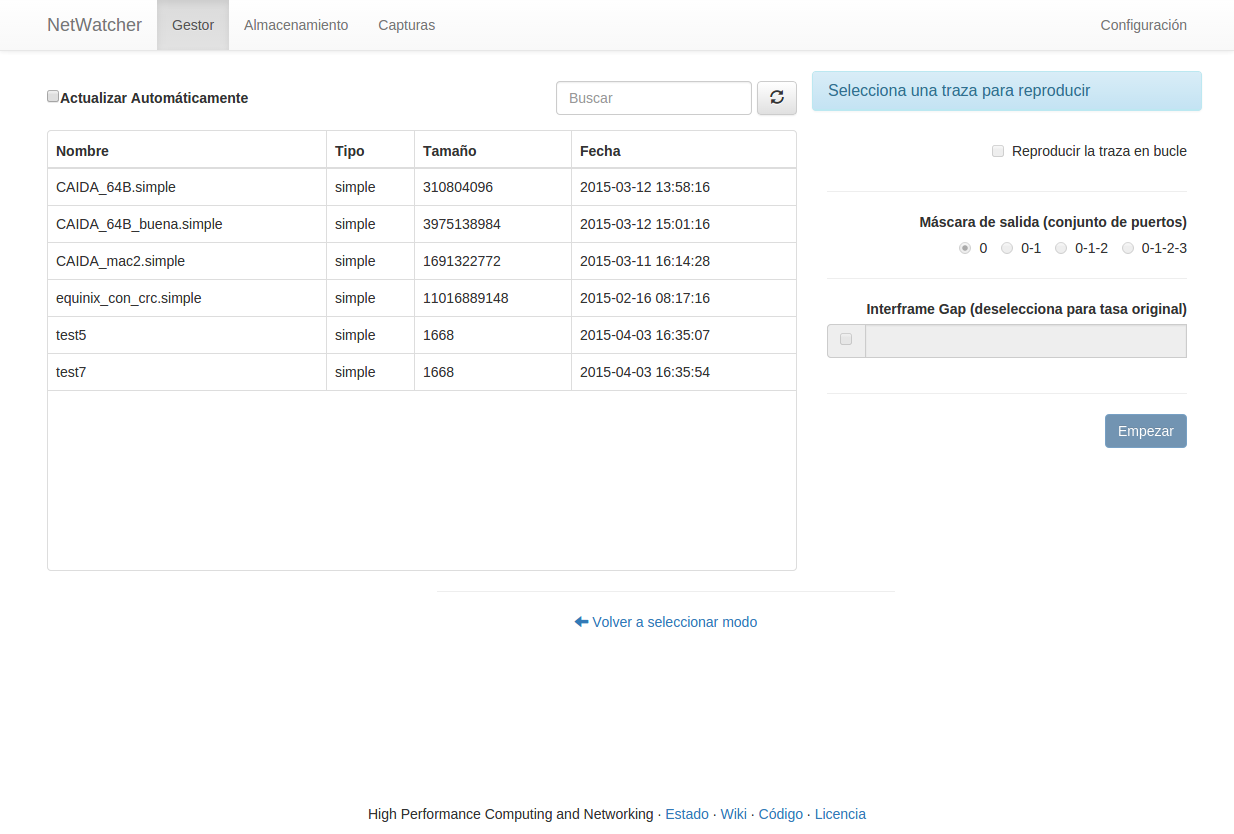
\includegraphics[width=\textwidth,clip=true]{graphics/capturas/gestor_reproducir}
  \caption{Página de gestión - reproducir \gls{traza}.}
  \label{fig:captura:gestionreproducir}
\end{figure}

Si la \gls{FPGA} está reproduciendo una \gls{traza}, la pantalla de gestión mostrará el progreso de la reproducción en curso (ver Figura \ref{fig:captura:gestionreproduciendo}). Se podrán visualizar las siguientes estadísticas de la reproducción en curso:
\begin{itemize}
  \item \textbf{Nombre de la \gls{traza}}: nombre de la \gls{traza} que se está reproduciendo.
  \item \textbf{Tamaño}: número de bytes que ocupa la \gls{traza} que se está reproduciendo.
  \item \textbf{Fecha}: fecha en que se creó la \gls{traza} que se está reproduciendo.
  \item \textbf{Tiempo Transcurrido}: contador del tiempo que ha transcurrido desde que se inició la captura.
  \item \textbf{Paquetes Enviados}: número de paquetes que se han enviado en la reproducción actual.
  \item \textbf{Reproducción en Bucle}: indica si se está reproduciendo la \gls{traza} en un bucle infinito o no.
  \item \textbf{Interframe Gap}: valor del \gls{IFG} en la reproducción actual.
  \item \textbf{Máscara}: conjunto de puertos en los que se está reproduciendo la \gls{traza} seleccionada (0, 0-1, 0-1-2, 0-1-2-3).
\end{itemize}

Se puede detener la reproducción en curso pulsando el botón \textit{Parar la reproducción}.

\begin{figure}[!htp]
  \centering
  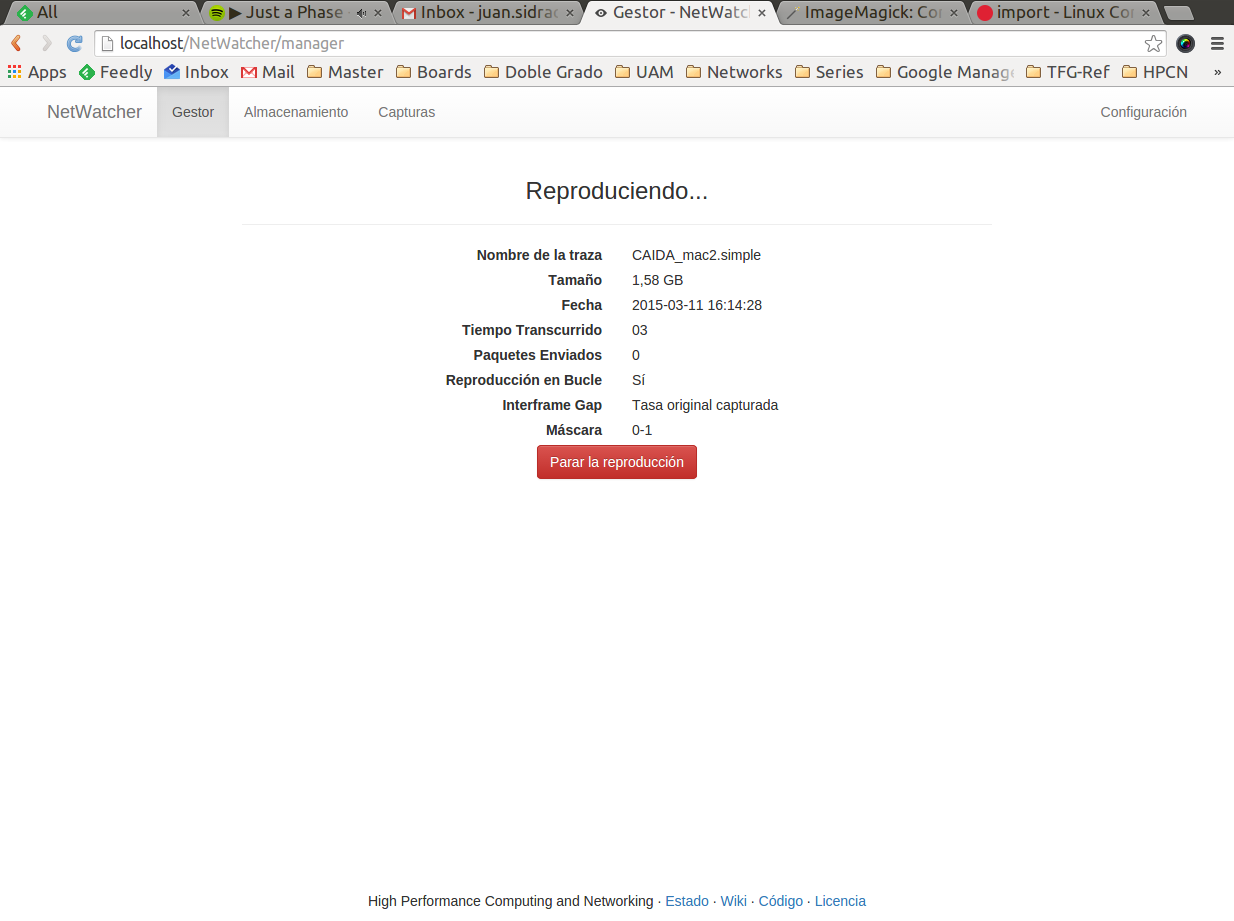
\includegraphics[width=\textwidth,clip=true]{graphics/capturas/gestor_reproduccion}
  \caption{Página de gestión - reproduciendo \gls{traza}.}
  \label{fig:captura:gestionreproduciendo}
\end{figure}


\subsection{Almacenamiento\label{extra:manual:almacenamiento}}

En esta pantalla se pueden visualizar distintas estadísticas de almacenamiento del sistema. Está compuesta por dos paneles:

\begin{itemize}
\item \textbf{Estadísticas de espacio (Figura \ref{fig:captura:espacio})}: este panel muestra estadísticas del espacio total, ocupado y disponible, resumido además en un gráfico circular (en rojo la proporción de disco ocupado y en turquesa la proporción de disco disponible).
\begin{figure}[!htp]
  \centering
  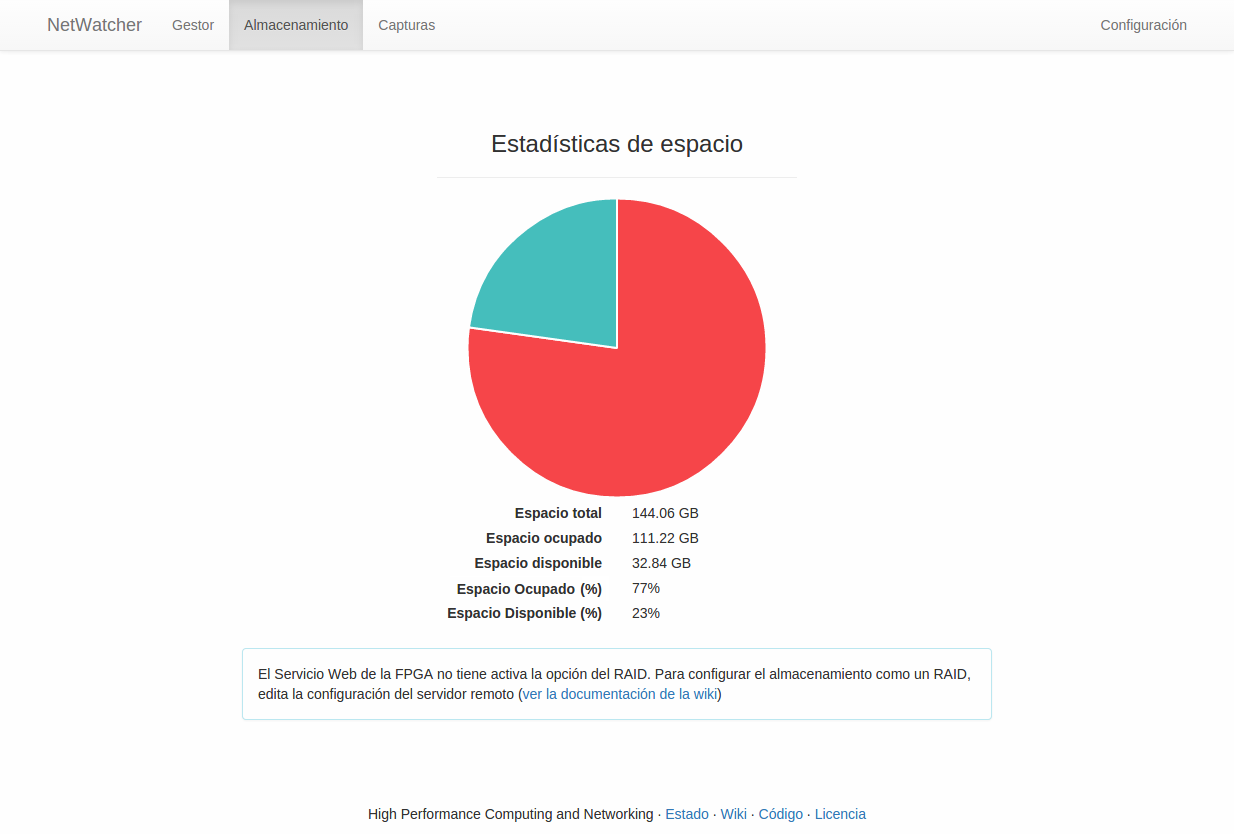
\includegraphics[width=\textwidth,clip=true]{graphics/capturas/almacenamiento_espacio}
  \caption{Página de almacenamiento, con \gls{RAID} no activo.}
  \label{fig:captura:espacio}
\end{figure}

\item \textbf{Estadísticas del \gls{RAID} (Figura \ref{fig:captura:raid})}: solo se mostrarán estas estadísticas si el sistema de almacenamiento está configurado como un \gls{RAID} (ver Sección \ref{extra:manual:configfpga}). En este panel, un gráfico de barras muestra la velocidad de escritura de cada disco del \gls{RAID}. Debajo de este gráfico se indica la velocidad global de escritura del \gls{RAID}. El color de esta cifra depende de la velocidad de escritura: verde (velocidad superior a la recomendada), amarillo (velocidad suficiente) o rojo (velocidad por debajo del mínimo aceptable). Si la velocidad es insuficiente se mostrará un cuadro de diálogo adicional para formatear y recrear el \gls{RAID} pulsando el botón \textit{Formatear el \gls{RAID}} (cuidado: formatear el \gls{RAID} borrará todos los datos del mismo). Este diálogo se puede ocultar pulsando el botón \textit{Descartar}.
\begin{figure}[!htp]
  \centering
  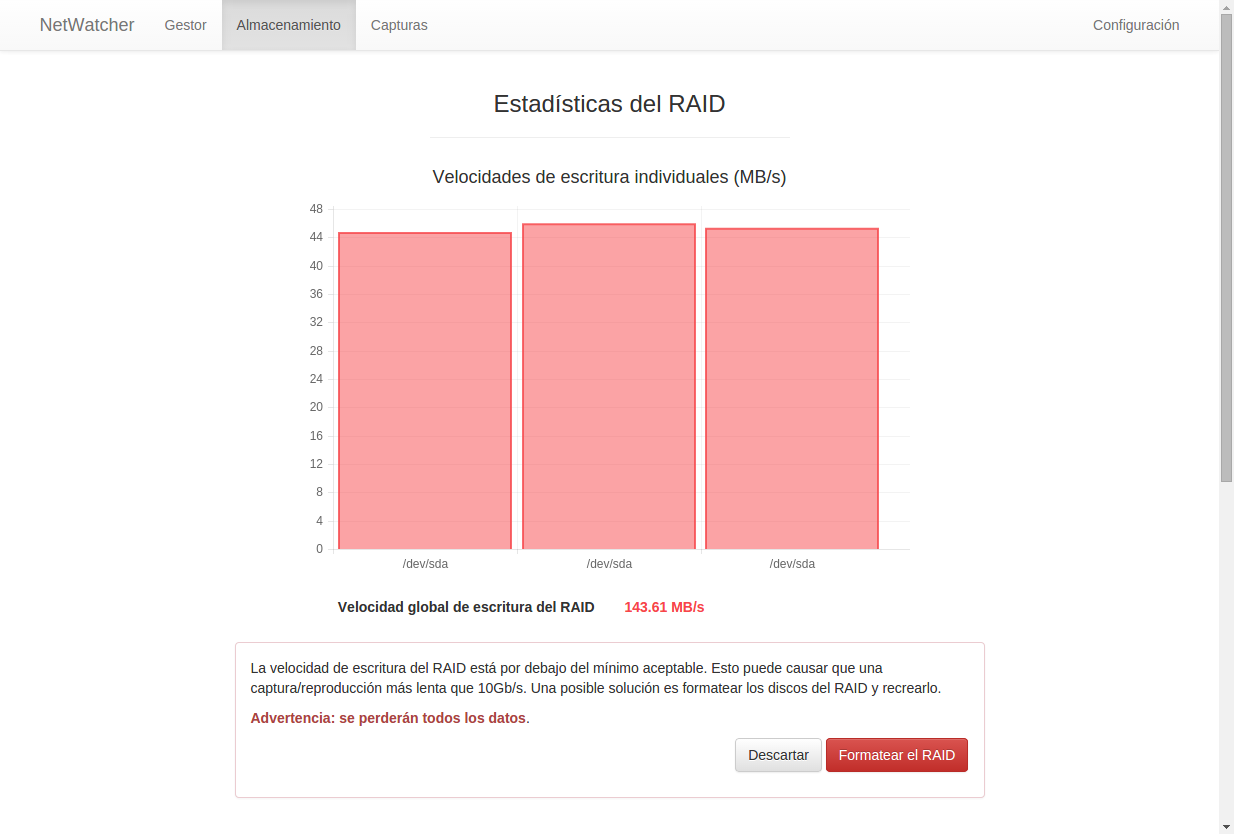
\includegraphics[width=\textwidth,clip=true]{graphics/capturas/almacenamiento_raid}
  \caption{Página de almacenamiento, con \gls{RAID} activo.}
  \label{fig:captura:raid}
\end{figure}
\end{itemize}


\subsection{Capturas\label{extra:manual:capturas}}

En esta pantalla se pueden gestionar las \glspl{traza} almacenadas (ver Figura \ref{fig:captura:capturas}), mediante una tabla y un panel de acciones. La tabla contiene una fila por cada \gls{traza} disponible, con su nombre, tipo, tamaño y fecha. Además, una barra superior asociada a esta tabla permite controlar el contenido de la misma mediante las siguientes acciones (de izquierda a derecha): filtrar las \glspl{traza} que se muestran según su tipo, activar la actualización automática de las \glspl{traza} disponibles, buscar una \gls{traza} por su nombre y actualizar manualmente las \glspl{traza} disponibles. Pulsando sobre una fila de la tabla se seleccionará la \gls{traza} correspondiente, activándose el panel de acciones. Este panel permite, mediante cada uno de sus subpaneles, las siguientes operaciones:
\begin{itemize}
  \item \textbf{Convertir}: crea una nueva \gls{traza} a partir de la \gls{traza} seleccionada cambiando el tipo (si la original tiene formato \gls{simple} la convertida tendrá formato \gls{pcap}, y viceversa).
  \item \textbf{Renombrar}: cambia el nombre de la \gls{traza} seleccionada al nuevo nombre introducido.
  \item \textbf{Borrar}: borra del disco la \gls{traza} seleccionada.
\end{itemize}

Los dos primeros subpaneles permitirán realizar su acción (se activará el correspondiente botón de \textit{OK}) cuando el campo de texto asociado a cada operación sea introducido correctamente.

\begin{figure}[!htp]
  \centering
  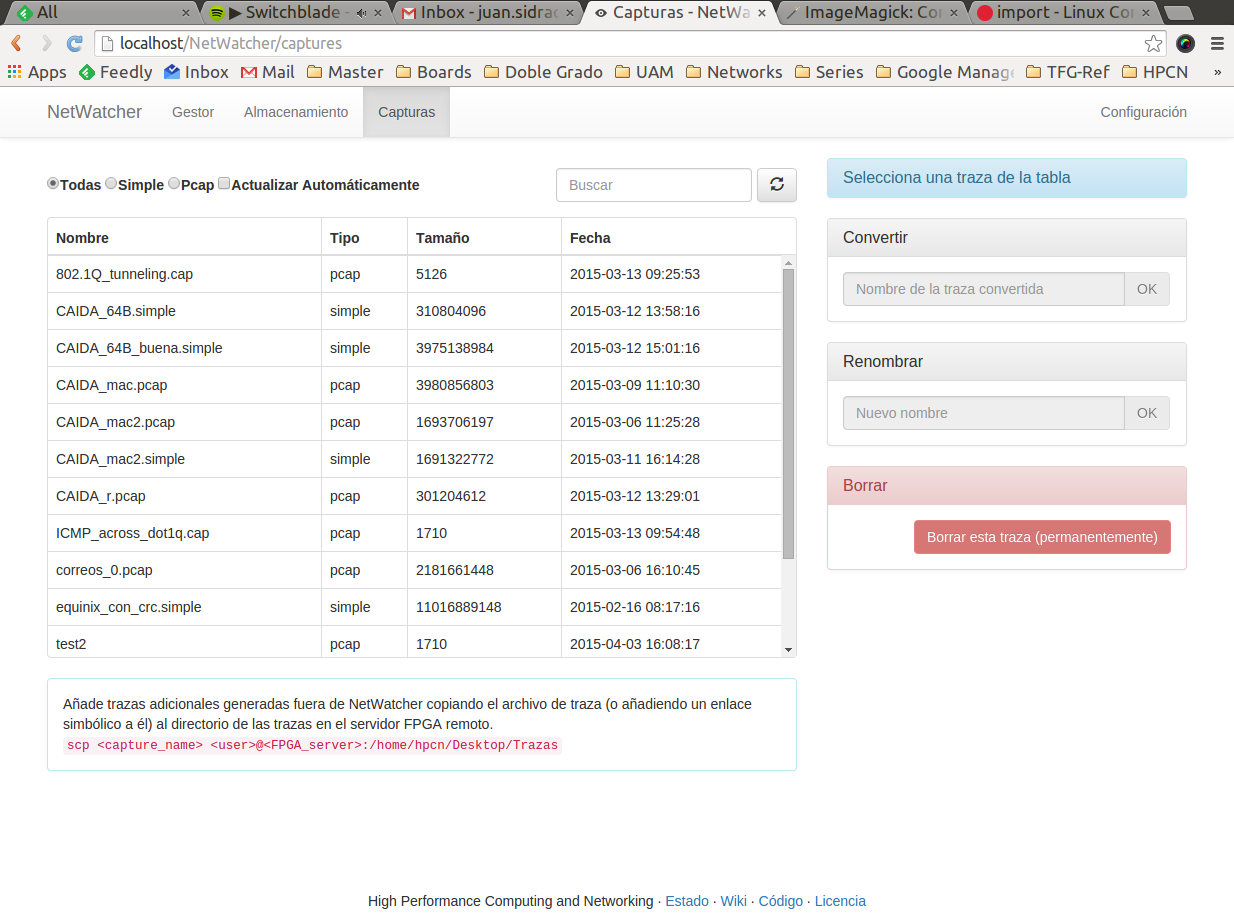
\includegraphics[width=\textwidth,clip=true]{graphics/capturas/capturas}
  \caption{Página de capturas.}
  \label{fig:captura:capturas}
\end{figure}


\subsection{Estado\label{extra:manual:estado}}

En esta pantalla se puede comprobar el estado de los distintos componentes que forman la aplicación (ver Figura \ref{fig:captura:estado}). Cada componente tiene un test asociado cuyo resultado se refleja en un panel. Cada test puede tener tres resultados distintos: \textit{OK} (test pasado, en verde), \textit{No Implementado} (test no implementado, en amarillo) y \textit{Error} (test fallado, en rojo). Los componentes sobre los que se comprueba su estado son los siguientes:
\begin{itemize}
  \item \textbf{Módulo Rewrite}: soporte para reescritura de \gls{URL}.
  \item \textbf{Módulo Gettext}: soporte para localización (traducción a distintos idiomas).
  \item \textbf{Variables de Sesión}: soporte para el uso de sesiones en \gls{PHP}.
  \item \textbf{Permisos de escritura}: permisos para escribir \textit{logs} y archivos de configuración.
  \item \textbf{Servidor Proxy}: servidor proxy habilitado para llamadas a la API \gls{FPGA}.
  \item \textbf{\gls{FPGA} API}: servidor de la \gls{FPGA} activo.
  \item \textbf{Relojes Sincronizados}: diferencia de relojes entre el cliente y el servidor \gls{FPGA} dentro del umbral permitido.
\end{itemize}

Adicionalmente, una barra de progreso encima de todo los paneles resume el estado global del sistema.

\begin{figure}[!htp]
  \centering
  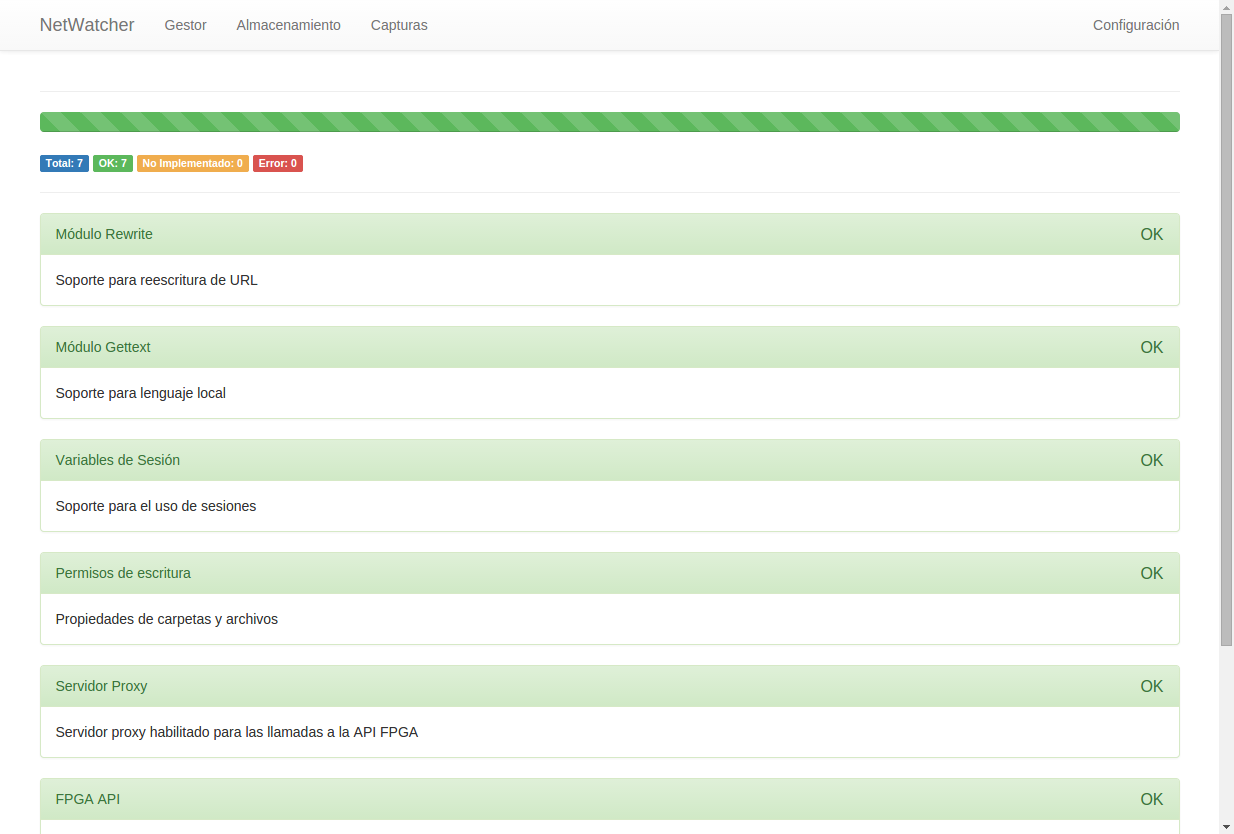
\includegraphics[width=\textwidth,clip=true]{graphics/capturas/estado}
  \caption{Página de estado del sistema.}
  \label{fig:captura:estado}
\end{figure}


\section{Solución de problemas\label{extra:manual:solucion}}

Si tras seguir las instrucciones paso a paso algo impide el correcto funcionamiento de la aplicación, se puede consultar la página de solución de problemas (en inglés), disponible dentro del repositorio del proyecto en:

\href{https://github.com/JSidrach/NetWatcher/blob/master/docs/wiki/Troubleshooting.md}{github.com/JSidrach/NetWatcher/blob/master/docs/wiki/Troubleshooting.md}